\section{Analysis strategy}
\label{sec:Durchführung}
This analysis is done with three data samples of which the invariant mass distributions are shown in \autoref{fig:dists}. Two of those contain Monte Carlo (MC) simulation of the $B^0_s \to \psi(2S)K^0_\mathrm{S}$ and the kinematically similar $B^0_d \to \to \psi(2S)K^0_\mathrm{S}$ decay, respectively. The third data sample contains data recorded by the LHCb experiment. The simulation of the $B^0_d$ decay will be used as a control channel.

\begin{figure}[tb]
  \centering
  \begin{subfigure}{.32\textwidth}
    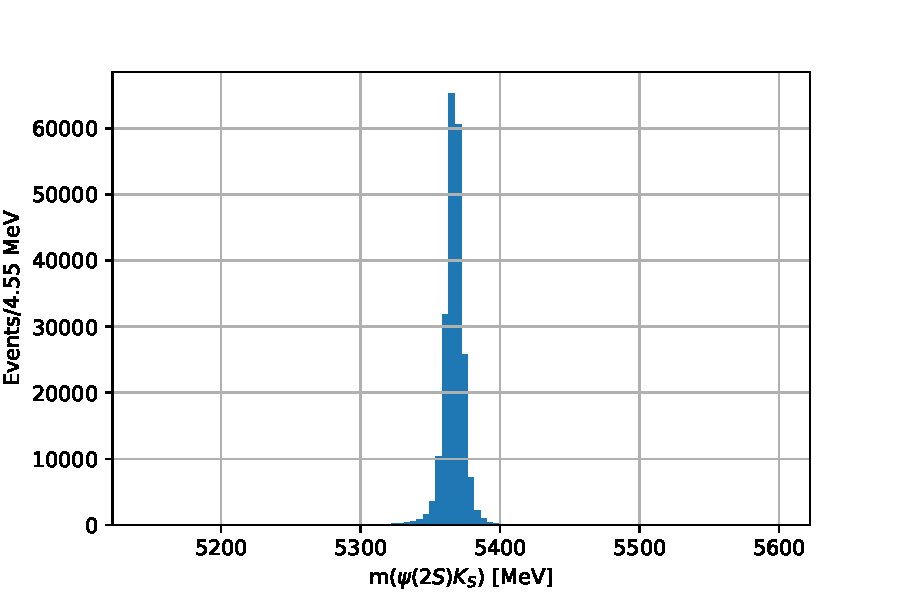
\includegraphics[width=\linewidth]{plots/sim_hist.pdf}
  \end{subfigure}
  \begin{subfigure}{.32\textwidth}
    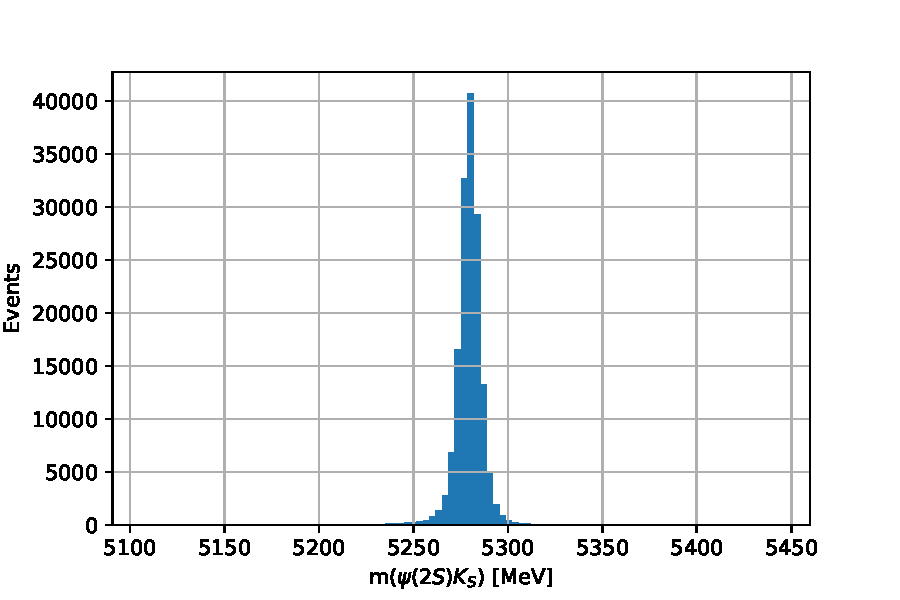
\includegraphics[width=\linewidth]{plots/control_sim_hist.pdf}
  \end{subfigure}
  \begin{subfigure}{.32\textwidth}
    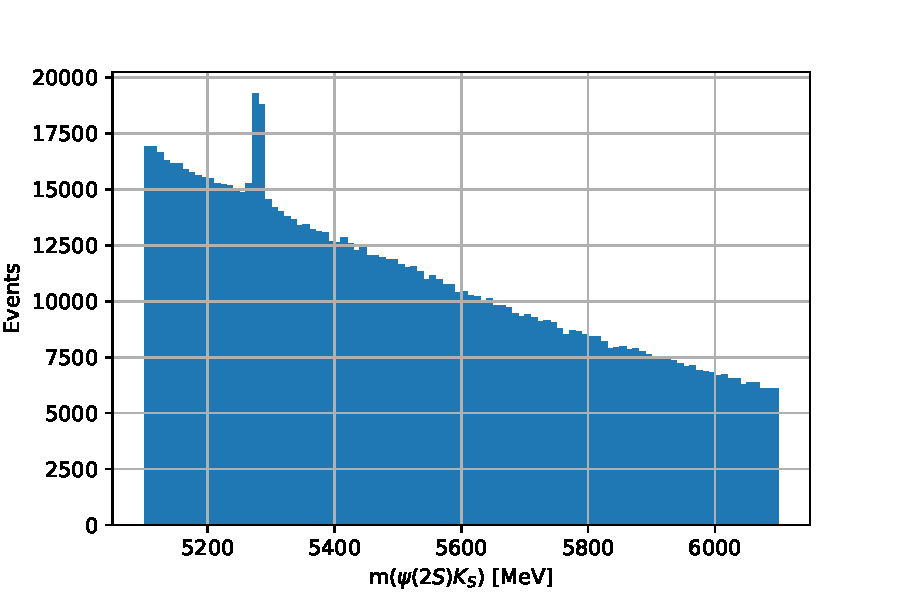
\includegraphics[width=\linewidth]{plots/data_hist.pdf}
  \end{subfigure}
  \caption{Invariant mass distributions of the MC simulated decays $B^0_s$ (left) and $B^0_d \to \psi(2S) K^0_\mathrm{S}$ (middle), as well as recorded data from the LHCb experiment (right).}
  \label{fig:dists}
\end{figure}

These are used to select a small number of features available that are similar in data and simulation and have a high separation power between signal and background. Those features are used to implement a BDT that serves as a multivariate classifier to reject as much combinatorial background as possible. A fit model is applied to the selected data from which the signal yield can be determined and the statistical significance can be estimated.
